\section{tasks::test Class Reference}
\label{classtasks_1_1test}\index{tasks::test@{tasks::test}}
Inheritance diagram for tasks::test::\begin{figure}[H]
\begin{center}
\leavevmode
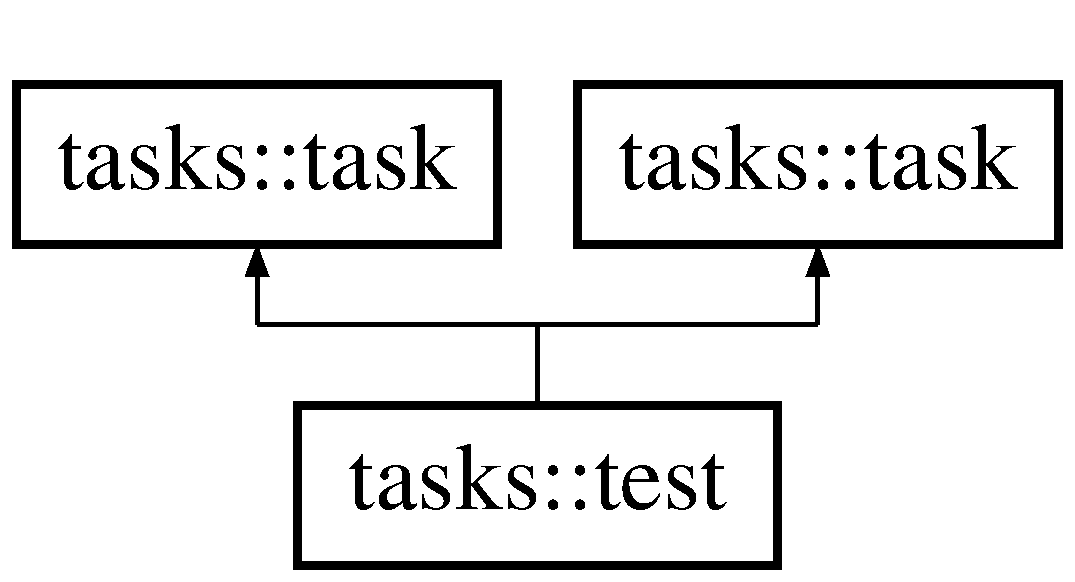
\includegraphics[height=2cm]{classtasks_1_1test}
\end{center}
\end{figure}
\subsection*{Public Member Functions}
\begin{CompactItemize}
\item 
def \textbf{\_\-\_\-init\_\-\_\-}\label{classtasks_1_1test_0cb323f022fd44123c950b76f061e776}

\item 
def \textbf{run}\label{classtasks_1_1test_798d0bc762bfddaef6de0058a4acf86f}

\item 
def \textbf{\_\-\_\-init\_\-\_\-}\label{classtasks_1_1test_0cb323f022fd44123c950b76f061e776}

\item 
def \textbf{run}\label{classtasks_1_1test_798d0bc762bfddaef6de0058a4acf86f}

\end{CompactItemize}
\subsection*{Static Public Attributes}
\begin{CompactItemize}
\item 
string \textbf{name} = '{\bftest}'\label{classtasks_1_1test_fedc868815b9ee3fcd3dde2b0acef22f}

\item 
string \textbf{button\-Text} = '{\bftest}'\label{classtasks_1_1test_d29763969e4128804e59324dee960c05}

\item 
int \textbf{inthread} = 0\label{classtasks_1_1test_d481510e691b04fbff713c2662a73c9e}

\end{CompactItemize}


\subsection{Detailed Description}


\footnotesize\begin{verbatim}Subtract two selected frames
\end{verbatim}
\normalsize
 



The documentation for this class was generated from the following files:\begin{CompactItemize}
\item 
old/PANICtool-1.0/tasks.py\item 
old/tasks.py\end{CompactItemize}
